% Options for packages loaded elsewhere
\PassOptionsToPackage{unicode}{hyperref}
\PassOptionsToPackage{hyphens}{url}
\documentclass[
]{book}
\usepackage{xcolor}
\usepackage{amsmath,amssymb}
\setcounter{secnumdepth}{5}
\usepackage{iftex}
\ifPDFTeX
  \usepackage[T1]{fontenc}
  \usepackage[utf8]{inputenc}
  \usepackage{textcomp} % provide euro and other symbols
\else % if luatex or xetex
  \usepackage{unicode-math} % this also loads fontspec
  \defaultfontfeatures{Scale=MatchLowercase}
  \defaultfontfeatures[\rmfamily]{Ligatures=TeX,Scale=1}
\fi
\usepackage{lmodern}
\ifPDFTeX\else
  % xetex/luatex font selection
\fi
% Use upquote if available, for straight quotes in verbatim environments
\IfFileExists{upquote.sty}{\usepackage{upquote}}{}
\IfFileExists{microtype.sty}{% use microtype if available
  \usepackage[]{microtype}
  \UseMicrotypeSet[protrusion]{basicmath} % disable protrusion for tt fonts
}{}
\makeatletter
\@ifundefined{KOMAClassName}{% if non-KOMA class
  \IfFileExists{parskip.sty}{%
    \usepackage{parskip}
  }{% else
    \setlength{\parindent}{0pt}
    \setlength{\parskip}{6pt plus 2pt minus 1pt}}
}{% if KOMA class
  \KOMAoptions{parskip=half}}
\makeatother
\usepackage{color}
\usepackage{fancyvrb}
\newcommand{\VerbBar}{|}
\newcommand{\VERB}{\Verb[commandchars=\\\{\}]}
\DefineVerbatimEnvironment{Highlighting}{Verbatim}{commandchars=\\\{\}}
% Add ',fontsize=\small' for more characters per line
\usepackage{framed}
\definecolor{shadecolor}{RGB}{248,248,248}
\newenvironment{Shaded}{\begin{snugshade}}{\end{snugshade}}
\newcommand{\AlertTok}[1]{\textcolor[rgb]{0.94,0.16,0.16}{#1}}
\newcommand{\AnnotationTok}[1]{\textcolor[rgb]{0.56,0.35,0.01}{\textbf{\textit{#1}}}}
\newcommand{\AttributeTok}[1]{\textcolor[rgb]{0.13,0.29,0.53}{#1}}
\newcommand{\BaseNTok}[1]{\textcolor[rgb]{0.00,0.00,0.81}{#1}}
\newcommand{\BuiltInTok}[1]{#1}
\newcommand{\CharTok}[1]{\textcolor[rgb]{0.31,0.60,0.02}{#1}}
\newcommand{\CommentTok}[1]{\textcolor[rgb]{0.56,0.35,0.01}{\textit{#1}}}
\newcommand{\CommentVarTok}[1]{\textcolor[rgb]{0.56,0.35,0.01}{\textbf{\textit{#1}}}}
\newcommand{\ConstantTok}[1]{\textcolor[rgb]{0.56,0.35,0.01}{#1}}
\newcommand{\ControlFlowTok}[1]{\textcolor[rgb]{0.13,0.29,0.53}{\textbf{#1}}}
\newcommand{\DataTypeTok}[1]{\textcolor[rgb]{0.13,0.29,0.53}{#1}}
\newcommand{\DecValTok}[1]{\textcolor[rgb]{0.00,0.00,0.81}{#1}}
\newcommand{\DocumentationTok}[1]{\textcolor[rgb]{0.56,0.35,0.01}{\textbf{\textit{#1}}}}
\newcommand{\ErrorTok}[1]{\textcolor[rgb]{0.64,0.00,0.00}{\textbf{#1}}}
\newcommand{\ExtensionTok}[1]{#1}
\newcommand{\FloatTok}[1]{\textcolor[rgb]{0.00,0.00,0.81}{#1}}
\newcommand{\FunctionTok}[1]{\textcolor[rgb]{0.13,0.29,0.53}{\textbf{#1}}}
\newcommand{\ImportTok}[1]{#1}
\newcommand{\InformationTok}[1]{\textcolor[rgb]{0.56,0.35,0.01}{\textbf{\textit{#1}}}}
\newcommand{\KeywordTok}[1]{\textcolor[rgb]{0.13,0.29,0.53}{\textbf{#1}}}
\newcommand{\NormalTok}[1]{#1}
\newcommand{\OperatorTok}[1]{\textcolor[rgb]{0.81,0.36,0.00}{\textbf{#1}}}
\newcommand{\OtherTok}[1]{\textcolor[rgb]{0.56,0.35,0.01}{#1}}
\newcommand{\PreprocessorTok}[1]{\textcolor[rgb]{0.56,0.35,0.01}{\textit{#1}}}
\newcommand{\RegionMarkerTok}[1]{#1}
\newcommand{\SpecialCharTok}[1]{\textcolor[rgb]{0.81,0.36,0.00}{\textbf{#1}}}
\newcommand{\SpecialStringTok}[1]{\textcolor[rgb]{0.31,0.60,0.02}{#1}}
\newcommand{\StringTok}[1]{\textcolor[rgb]{0.31,0.60,0.02}{#1}}
\newcommand{\VariableTok}[1]{\textcolor[rgb]{0.00,0.00,0.00}{#1}}
\newcommand{\VerbatimStringTok}[1]{\textcolor[rgb]{0.31,0.60,0.02}{#1}}
\newcommand{\WarningTok}[1]{\textcolor[rgb]{0.56,0.35,0.01}{\textbf{\textit{#1}}}}
\usepackage{longtable,booktabs,array}
\usepackage{calc} % for calculating minipage widths
% Correct order of tables after \paragraph or \subparagraph
\usepackage{etoolbox}
\makeatletter
\patchcmd\longtable{\par}{\if@noskipsec\mbox{}\fi\par}{}{}
\makeatother
% Allow footnotes in longtable head/foot
\IfFileExists{footnotehyper.sty}{\usepackage{footnotehyper}}{\usepackage{footnote}}
\makesavenoteenv{longtable}
\usepackage{graphicx}
\makeatletter
\newsavebox\pandoc@box
\newcommand*\pandocbounded[1]{% scales image to fit in text height/width
  \sbox\pandoc@box{#1}%
  \Gscale@div\@tempa{\textheight}{\dimexpr\ht\pandoc@box+\dp\pandoc@box\relax}%
  \Gscale@div\@tempb{\linewidth}{\wd\pandoc@box}%
  \ifdim\@tempb\p@<\@tempa\p@\let\@tempa\@tempb\fi% select the smaller of both
  \ifdim\@tempa\p@<\p@\scalebox{\@tempa}{\usebox\pandoc@box}%
  \else\usebox{\pandoc@box}%
  \fi%
}
% Set default figure placement to htbp
\def\fps@figure{htbp}
\makeatother
\setlength{\emergencystretch}{3em} % prevent overfull lines
\providecommand{\tightlist}{%
  \setlength{\itemsep}{0pt}\setlength{\parskip}{0pt}}
\usepackage[]{natbib}
\bibliographystyle{apalike}
\usepackage{booktabs}
\usepackage{bookmark}
\IfFileExists{xurl.sty}{\usepackage{xurl}}{} % add URL line breaks if available
\urlstyle{same}
\hypersetup{
  pdftitle={PSY 607 Bayesian Analysis},
  pdfauthor={Sara Weston},
  hidelinks,
  pdfcreator={LaTeX via pandoc}}

\title{PSY 607 Bayesian Analysis}
\author{Sara Weston}
\date{Spring 2025}

\begin{document}
\maketitle

{
\setcounter{tocdepth}{1}
\tableofcontents
}
\chapter{Course description}\label{course-description}

\section{Structure}\label{structure}

\section{Materials}\label{materials}

\section{Schedule}\label{schedule}

\section{Grades}\label{grades}

\section{Policies}\label{policies}

\subsection{Abscences}\label{abscences}

\subsection{Communication}\label{communication}

If you have questions about course policies, have trouble submitting an assignment, or want to schedule a meeting, please email. I will make an effort to respond to emails within one business day. Note that I neither plan nor commit to checking email outside of normal business hours (9am-5pm, Mon-Fri).

If you are having trouble understanding a concept covered in class, please come to office hours, schedule a meeting with me, or ask for clarification during class periods. I will not explain course concepts over email.

Occasionally, I will send out announcements to the entire class via Canvas announcements. These will typically appear when you open Canvas, but you can update your Canvas settings to receive these announcements as emails. It is strongly recommended that you do so.

\subsection{Classroom}\label{classroom}

All members of the class (students and instructor) can expect to:

\emph{Participate and Contribute:} All students are expected to participate by sharing ideas and contributing to the learning environment. This entails preparing, following instructions, and engaging respectfully and thoughtfully with others.

While all students should participate, participation is not just talking, and a range of participation activities support learning. Participation might look like speaking aloud in the full class and in small groups and collaborating on homework assignments.

\emph{Expect and Respect Diversity:} All classes at the University of Oregon welcome and respect diverse experiences, perspectives, and approaches. What is not welcome are behaviors or contributions that undermine, demean, or marginalize others based on race, ethnicity, gender, sex, age, sexual orientation, religion, ability, or socioeconomic status. We will value differences and communicate disagreements with respect.

\emph{Help Everyone Learn:} Part of how we learn together is by learning from one another. To do this effectively, we need to be patient with each other, identify ways we can assist others, and be open-minded to receiving help and feedback from others. Don't hesitate to contact me to ask for assistance or offer suggestions that might help us learn better.

\subsection{Workload}\label{workload}

This is a 3-credit hour course, so you should expect to complete 120 hours of work for the course---an average of about 12 hours each week (this includes time in-class).

\subsection{Generative AI}\label{generative-ai}

\subsection{Plagiarism}\label{plagiarism}

\subsection{Accessibility}\label{accessibility}

\subsection{Basic needs}\label{basic-needs}

\subsection{Reporting obligations}\label{reporting-obligations}

\subsection{Campus emergencies}\label{campus-emergencies}

\chapter{Week 1: Introduction to Bayesian Analysis}\label{week-1-introduction-to-bayesian-analysis}

\section{Class 1: Probability}\label{class-1-probability}

\subsection{Slides}\label{slides}

This lecture is based on the following article: \citet{etz_introduction_2018-1}. \href{readings/Etz\%20and\%20Vandekerckhove\%20-\%202018\%20-\%20Introduction\%20to\%20Bayesian\%20Inference\%20for\%20Psychology.pdf}{download here.}

\section{Class 2: Bayes as counting}\label{class-2-bayes-as-counting}

Before class, be sure to watch both of the following lectures by McElreath:
* \href{Science\%20Before\%20Statistics}{Science before statistics}
* \href{https://www.youtube.com/watch?v=R1vcdhPBlXA&list=PLDcUM9US4XdPz-KxHM4XHt7uUVGWWVSus&index=2}{Garden of forking data}

This lecture is based on Chapters 2 and 3 in \emph{Statistical Rethinking} by Richard McElreath.

\chapter{Week 2: Linear models and causal inference}\label{week-2-linear-models-and-causal-inference}

\section{Class 1: Geocentric models}\label{class-1-geocentric-models}

Before class, be sure to \href{https://www.youtube.com/watch?v=tNOu-SEacNU&list=PLDcUM9US4XdPz-KxHM4XHt7uUVGWWVSus&index=3}{watch the lecture by McElreath}.

\subsection{Slides}\label{slides-1}

This lecture is based on Chapters 4 in \emph{Statistical Rethinking} by Richard McElreath.

\section{Class 2: Categories (and curves)}\label{class-2-categories-and-curves}

Before class, be sure to \href{https://www.youtube.com/watch?v=F0N4b7K_iYQ&list=PLDcUM9US4XdPz-KxHM4XHt7uUVGWWVSus&index=4}{watch the lecture by McElreath}.

\subsection{Slides}\label{slides-2}

This lecture is based on Chapters 4 and 5 in \emph{Statistical Rethinking} by Richard McElreath.

\subsection{Curves (splines)}\label{curves-splines}

We won't have time to address curves in class, and McElreath doesn't give you a lot of code to work with in the lecture. Here's how to reproduce his spline model from the lecture.

\subsubsection{Data preparation}\label{data-preparation}

\begin{Shaded}
\begin{Highlighting}[]
\FunctionTok{library}\NormalTok{(rethinking)}
\FunctionTok{library}\NormalTok{(psych)}
\FunctionTok{library}\NormalTok{(tidyverse)}
\FunctionTok{library}\NormalTok{(splines)}
\end{Highlighting}
\end{Shaded}

\begin{Shaded}
\begin{Highlighting}[]
\FunctionTok{data}\NormalTok{(cherry\_blossoms)}
\NormalTok{d }\OtherTok{\textless{}{-}}\NormalTok{ cherry\_blossoms}
\FunctionTok{precis}\NormalTok{(d)}
\end{Highlighting}
\end{Shaded}

\begin{verbatim}
##                   mean          sd      5.5%      94.5%       histogram
## year       1408.000000 350.8845964 867.77000 1948.23000   ▇▇▇▇▇▇▇▇▇▇▇▇▁
## doy         104.540508   6.4070362  94.43000  115.00000        ▁▂▅▇▇▃▁▁
## temp          6.141886   0.6636479   5.15000    7.29470        ▁▃▅▇▃▂▁▁
## temp_upper    7.185151   0.9929206   5.89765    8.90235 ▁▂▅▇▇▅▂▂▁▁▁▁▁▁▁
## temp_lower    5.098941   0.8503496   3.78765    6.37000 ▁▁▁▁▁▁▁▃▅▇▃▂▁▁▁
\end{verbatim}

\begin{Shaded}
\begin{Highlighting}[]
\NormalTok{psych}\SpecialCharTok{::}\FunctionTok{describe}\NormalTok{(d)}
\end{Highlighting}
\end{Shaded}

\begin{verbatim}
##            vars    n    mean     sd  median trimmed    mad    min     max
## year          1 1215 1408.00 350.88 1408.00 1408.00 450.71 801.00 2015.00
## doy           2  827  104.54   6.41  105.00  104.54   5.93  86.00  124.00
## temp          3 1124    6.14   0.66    6.10    6.11   0.61   4.67    8.30
## temp_upper    4 1124    7.19   0.99    7.04    7.10   0.92   5.45   12.10
## temp_lower    5 1124    5.10   0.85    5.14    5.10   0.72   0.75    7.74
##              range  skew kurtosis    se
## year       1214.00  0.00    -1.20 10.07
## doy          38.00  0.00    -0.15  0.22
## temp          3.63  0.40     0.11  0.02
## temp_upper    6.65  1.05     1.71  0.03
## temp_lower    6.99 -0.17     1.88  0.03
\end{verbatim}

Note that some of the values for \texttt{doy} (day of year) are missing. The \texttt{quap()} function can't handle missingness, so we'll remove those rows before proceeding.

\begin{Shaded}
\begin{Highlighting}[]
\NormalTok{d2 }\OtherTok{\textless{}{-}}\NormalTok{ d[ }\FunctionTok{complete.cases}\NormalTok{(d}\SpecialCharTok{$}\NormalTok{doy) , ] }\CommentTok{\# complete cases on doy}
\end{Highlighting}
\end{Shaded}

Next we set up an arbitrary number of knots. Knots divide our data into \(N_{knots}+1\) equal bins, such that each bin has the same number of data points. McElreath chooses 15 knots.

\begin{Shaded}
\begin{Highlighting}[]
\NormalTok{num\_knots }\OtherTok{\textless{}{-}} \DecValTok{15}
\NormalTok{knot\_list }\OtherTok{\textless{}{-}} \FunctionTok{quantile}\NormalTok{( d2}\SpecialCharTok{$}\NormalTok{year , }\AttributeTok{probs=}\FunctionTok{seq}\NormalTok{(}\DecValTok{0}\NormalTok{,}\DecValTok{1}\NormalTok{,}\AttributeTok{length.out=}\NormalTok{num\_knots) )}
\NormalTok{knot\_list}
\end{Highlighting}
\end{Shaded}

\begin{verbatim}
##        0% 7.142857% 14.28571% 21.42857% 28.57143% 35.71429% 42.85714%       50% 
##       812      1036      1174      1269      1377      1454      1518      1583 
## 57.14286% 64.28571% 71.42857% 78.57143% 85.71429% 92.85714%      100% 
##      1650      1714      1774      1833      1893      1956      2015
\end{verbatim}

To visualize how our data have been partitioned:

\begin{Shaded}
\begin{Highlighting}[]
\NormalTok{d2 }\SpecialCharTok{\%\textgreater{}\%} 
  \FunctionTok{ggplot}\NormalTok{(}\FunctionTok{aes}\NormalTok{(}\AttributeTok{x =}\NormalTok{ year, }\AttributeTok{y =}\NormalTok{ doy)) }\SpecialCharTok{+}
  \FunctionTok{geom\_point}\NormalTok{(}\AttributeTok{color =} \StringTok{"\#ffb7c5"}\NormalTok{, }\AttributeTok{alpha =} \DecValTok{1}\SpecialCharTok{/}\DecValTok{2}\NormalTok{) }\SpecialCharTok{+} 
  \FunctionTok{geom\_vline}\NormalTok{(}\AttributeTok{xintercept =}\NormalTok{ knot\_list, }\AttributeTok{color =} \StringTok{"white"}\NormalTok{, }\AttributeTok{alpha =}\NormalTok{ .}\DecValTok{5}\NormalTok{) }\SpecialCharTok{+}
  \FunctionTok{theme}\NormalTok{(}\AttributeTok{panel.grid =} \FunctionTok{element\_blank}\NormalTok{(),}
        \AttributeTok{panel.background =} \FunctionTok{element\_rect}\NormalTok{(}\AttributeTok{fill =} \StringTok{"\#4f455c"}\NormalTok{))}
\end{Highlighting}
\end{Shaded}

\pandocbounded{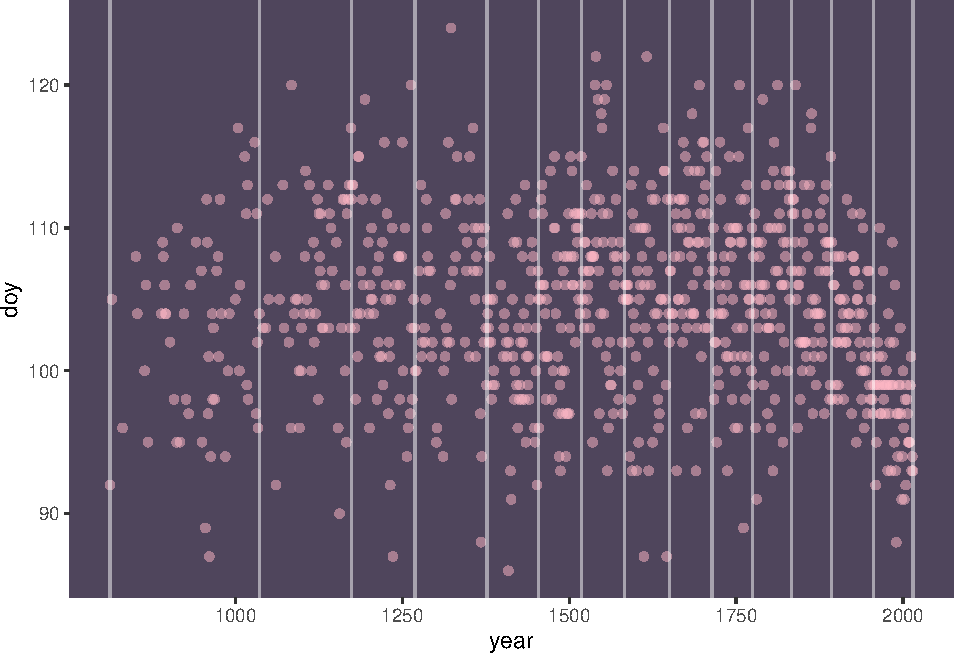
\includegraphics[keepaspectratio]{_main_files/figure-latex/unnamed-chunk-6-1.pdf}}

Next, we'll use functions in the \texttt{spline} package to create basis spline functions based on these knots

\begin{Shaded}
\begin{Highlighting}[]
\NormalTok{B }\OtherTok{\textless{}{-}} \FunctionTok{bs}\NormalTok{(d2}\SpecialCharTok{$}\NormalTok{year,}
  \AttributeTok{knots=}\NormalTok{knot\_list[}\SpecialCharTok{{-}}\FunctionTok{c}\NormalTok{(}\DecValTok{1}\NormalTok{,num\_knots)] ,}
  \AttributeTok{degree=}\DecValTok{3}\NormalTok{ , }\AttributeTok{intercept=}\ConstantTok{TRUE}\NormalTok{ )}

\FunctionTok{plot}\NormalTok{( }\ConstantTok{NULL}\NormalTok{ , }\AttributeTok{xlim=}\FunctionTok{range}\NormalTok{(d2}\SpecialCharTok{$}\NormalTok{year) , }\AttributeTok{ylim=}\FunctionTok{c}\NormalTok{(}\DecValTok{0}\NormalTok{,}\DecValTok{1}\NormalTok{) , }\AttributeTok{xlab=}\StringTok{"year"}\NormalTok{ , }\AttributeTok{ylab=}\StringTok{"basis"}\NormalTok{ )}
\ControlFlowTok{for}\NormalTok{ ( i }\ControlFlowTok{in} \DecValTok{1}\SpecialCharTok{:}\FunctionTok{ncol}\NormalTok{(B) ) }\FunctionTok{lines}\NormalTok{( d2}\SpecialCharTok{$}\NormalTok{year , B[,i] )}
\end{Highlighting}
\end{Shaded}

\pandocbounded{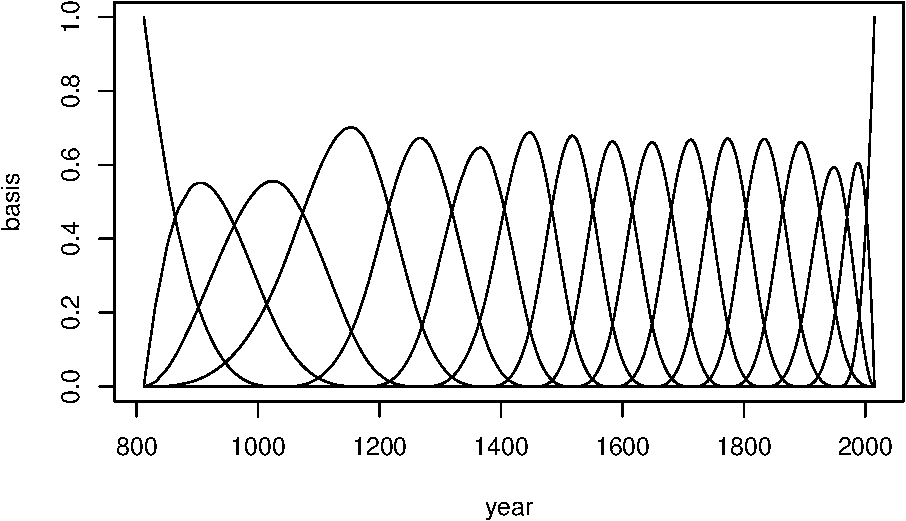
\includegraphics[keepaspectratio]{_main_files/figure-latex/unnamed-chunk-7-1.pdf}}

\subsubsection{\texorpdfstring{Mathematical model and \texttt{quap()}}{Mathematical model and quap()}}\label{mathematical-model-and-quap}

Here is the mathematical model for the spline model:

\begin{align*}
D_i &\sim \text{Normal}(\mu_i,\sigma) \\
\mu_i &= \alpha + \sum^K_{k=1} w_k B_{k,i} \\
\alpha &\sim \text{Normal}(100,10) \\
w_j &\sim \text{Normal}(0,10) \\
\sigma &\sim \text{Exponential}(1)
\end{align*}

And here's how we can fit this using \texttt{quap()}. Note that this is the first use of the \texttt{start} function, which gives the estimation algorithm a start value. This can be helpful if you find that models are not converging.

\begin{Shaded}
\begin{Highlighting}[]
\NormalTok{m5}\OtherTok{\textless{}{-}} \FunctionTok{quap}\NormalTok{(}

  \FunctionTok{alist}\NormalTok{(}
\NormalTok{  D }\SpecialCharTok{\textasciitilde{}} \FunctionTok{dnorm}\NormalTok{( mu , sigma ) ,}
\NormalTok{  mu }\OtherTok{\textless{}{-}}\NormalTok{ a }\SpecialCharTok{+}\NormalTok{ B }\SpecialCharTok{\%*\%}\NormalTok{ w ,}
\NormalTok{  a }\SpecialCharTok{\textasciitilde{}} \FunctionTok{dnorm}\NormalTok{(}\DecValTok{100}\NormalTok{,}\DecValTok{10}\NormalTok{),}
\NormalTok{  w }\SpecialCharTok{\textasciitilde{}} \FunctionTok{dnorm}\NormalTok{(}\DecValTok{0}\NormalTok{,}\DecValTok{10}\NormalTok{),}
\NormalTok{  sigma }\SpecialCharTok{\textasciitilde{}} \FunctionTok{dexp}\NormalTok{(}\DecValTok{1}\NormalTok{)), }
  
  \AttributeTok{data=}\FunctionTok{list}\NormalTok{( }\AttributeTok{D=}\NormalTok{d2}\SpecialCharTok{$}\NormalTok{doy , }\AttributeTok{B=}\NormalTok{B ) ,}
  
  \AttributeTok{start=}\FunctionTok{list}\NormalTok{( }\AttributeTok{w=}\FunctionTok{rep}\NormalTok{( }\DecValTok{0}\NormalTok{ , }\FunctionTok{ncol}\NormalTok{(B) ) ) )}
\end{Highlighting}
\end{Shaded}

\chapter{Week 3: Causes, Confounds, and Colliders}\label{week-3-causes-confounds-and-colliders}

\section{Class 1: Elemental confounds}\label{class-1-elemental-confounds}

Before class, be sure to \href{https://www.youtube.com/watch?v=mBEA7PKDmiY&list=PLDcUM9US4XdPz-KxHM4XHt7uUVGWWVSus&index=5}{watch the lecture by McElreath}.

\subsection{Slides}\label{slides-3}

This lecture is based on Chapters 5 and 6 in \emph{Statistical Rethinking} by Richard McElreath.

You'll also want this code to simulate some fake plant data in class.

\begin{Shaded}
\begin{Highlighting}[]
\FunctionTok{set.seed}\NormalTok{(}\DecValTok{71}\NormalTok{)}
\CommentTok{\# number of plants}
\NormalTok{N }\OtherTok{\textless{}{-}} \DecValTok{100}
\CommentTok{\# simulate initial heights}
\NormalTok{h0 }\OtherTok{\textless{}{-}} \FunctionTok{rnorm}\NormalTok{(N,}\DecValTok{10}\NormalTok{,}\DecValTok{2}\NormalTok{)}
\CommentTok{\# assign treatments and simulate fungus and growth}
\NormalTok{treatment }\OtherTok{\textless{}{-}} \FunctionTok{rep}\NormalTok{( }\DecValTok{0}\SpecialCharTok{:}\DecValTok{1}\NormalTok{ , }\AttributeTok{each=}\NormalTok{N}\SpecialCharTok{/}\DecValTok{2}\NormalTok{ )}
\NormalTok{fungus }\OtherTok{\textless{}{-}} \FunctionTok{rbinom}\NormalTok{( N , }\AttributeTok{size=}\DecValTok{1}\NormalTok{ , }\AttributeTok{prob=}\FloatTok{0.5} \SpecialCharTok{{-}}\NormalTok{ treatment}\SpecialCharTok{*}\FloatTok{0.4}\NormalTok{ )}
\NormalTok{h1 }\OtherTok{\textless{}{-}}\NormalTok{ h0 }\SpecialCharTok{+} \FunctionTok{rnorm}\NormalTok{(N, }\DecValTok{5} \SpecialCharTok{{-}} \DecValTok{3}\SpecialCharTok{*}\NormalTok{fungus)}
\CommentTok{\# compose a clean data frame}
\NormalTok{d }\OtherTok{\textless{}{-}} \FunctionTok{data.frame}\NormalTok{( }\AttributeTok{h0=}\NormalTok{h0 , }\AttributeTok{h1=}\NormalTok{h1 , }\AttributeTok{treatment=}\NormalTok{treatment , }\AttributeTok{fungus=}\NormalTok{fungus )}
\end{Highlighting}
\end{Shaded}

\section{Class 2: Categories (and curves)}\label{class-2-categories-and-curves-1}

Before class, be sure to \href{https://www.youtube.com/watch?v=F0N4b7K_iYQ&list=PLDcUM9US4XdPz-KxHM4XHt7uUVGWWVSus&index=6}{watch the lecture by McElreath}.

\subsection{Slides}\label{slides-4}

This lecture is based on Chapter 6 in \emph{Statistical Rethinking} by Richard McElreath.

\subsection{Simulation Code}\label{simulation-code}

\subsubsection{Simulation 1: Simple Confounding}\label{simulation-1-simple-confounding}

In this code, the true causal effect of X on Y is 0, but confounded by U.

\begin{Shaded}
\begin{Highlighting}[]
\CommentTok{\#number of sims}
\NormalTok{N }\OtherTok{=} \DecValTok{1000}
\CommentTok{\# Generate data}
\NormalTok{U }\OtherTok{\textless{}{-}} \FunctionTok{rnorm}\NormalTok{(N)  }\CommentTok{\# Unobserved confounder}
\NormalTok{X }\OtherTok{\textless{}{-}} \FunctionTok{rnorm}\NormalTok{(N, }\AttributeTok{mean =} \FloatTok{0.5} \SpecialCharTok{*}\NormalTok{ U)  }\CommentTok{\# Treatment affected by U}
\NormalTok{Y }\OtherTok{\textless{}{-}} \FunctionTok{rnorm}\NormalTok{(N, }\AttributeTok{mean =} \FloatTok{0.8} \SpecialCharTok{*}\NormalTok{ U)  }\CommentTok{\# Outcome affected by U}
\NormalTok{Z }\OtherTok{\textless{}{-}} \FunctionTok{rnorm}\NormalTok{(N, }\AttributeTok{mean =} \FloatTok{0.6} \SpecialCharTok{*}\NormalTok{ U)  }\CommentTok{\# Observed variable that captures U}

\NormalTok{d }\OtherTok{\textless{}{-}} \FunctionTok{data.frame}\NormalTok{(X, Y, Z)}

\CommentTok{\# Fit models}
\NormalTok{flist1 }\OtherTok{\textless{}{-}} \FunctionTok{alist}\NormalTok{(}
\NormalTok{  Y }\SpecialCharTok{\textasciitilde{}} \FunctionTok{dnorm}\NormalTok{(mu, sigma),}
\NormalTok{  mu }\OtherTok{\textless{}{-}}\NormalTok{ a }\SpecialCharTok{+}\NormalTok{ bX}\SpecialCharTok{*}\NormalTok{X,}
\NormalTok{  a }\SpecialCharTok{\textasciitilde{}} \FunctionTok{dnorm}\NormalTok{(}\DecValTok{0}\NormalTok{, .}\DecValTok{5}\NormalTok{),}
\NormalTok{  bX }\SpecialCharTok{\textasciitilde{}} \FunctionTok{dnorm}\NormalTok{(}\DecValTok{0}\NormalTok{, .}\DecValTok{25}\NormalTok{),}
\NormalTok{  sigma }\SpecialCharTok{\textasciitilde{}} \FunctionTok{dexp}\NormalTok{(}\DecValTok{1}\NormalTok{)}
\NormalTok{)}

\NormalTok{m32}\FloatTok{.1} \OtherTok{\textless{}{-}} \FunctionTok{quap}\NormalTok{(flist1, d)}
\FunctionTok{precis}\NormalTok{(m32}\FloatTok{.1}\NormalTok{)}

\CommentTok{\# Fit models}
\NormalTok{flist2 }\OtherTok{\textless{}{-}} \FunctionTok{alist}\NormalTok{(}
\NormalTok{  Y }\SpecialCharTok{\textasciitilde{}} \FunctionTok{dnorm}\NormalTok{(mu, sigma),}
\NormalTok{  mu }\OtherTok{\textless{}{-}}\NormalTok{ a }\SpecialCharTok{+}\NormalTok{ bX}\SpecialCharTok{*}\NormalTok{X }\SpecialCharTok{+}\NormalTok{bZ}\SpecialCharTok{*}\NormalTok{Z,}
\NormalTok{  a }\SpecialCharTok{\textasciitilde{}} \FunctionTok{dnorm}\NormalTok{(}\DecValTok{0}\NormalTok{, .}\DecValTok{5}\NormalTok{),}
\NormalTok{  bX }\SpecialCharTok{\textasciitilde{}} \FunctionTok{dnorm}\NormalTok{(}\DecValTok{0}\NormalTok{, .}\DecValTok{25}\NormalTok{),}
\NormalTok{  bZ }\SpecialCharTok{\textasciitilde{}} \FunctionTok{dnorm}\NormalTok{(}\DecValTok{0}\NormalTok{, .}\DecValTok{25}\NormalTok{),}
\NormalTok{  sigma }\SpecialCharTok{\textasciitilde{}} \FunctionTok{dexp}\NormalTok{(}\DecValTok{1}\NormalTok{)}
\NormalTok{)}

\NormalTok{m32}\FloatTok{.2} \OtherTok{\textless{}{-}} \FunctionTok{quap}\NormalTok{(flist2, d)}
\FunctionTok{precis}\NormalTok{(m32}\FloatTok{.2}\NormalTok{)}

\NormalTok{post}\FloatTok{.1} \OtherTok{\textless{}{-}} \FunctionTok{extract.samples}\NormalTok{(m32}\FloatTok{.1}\NormalTok{)}
\NormalTok{post}\FloatTok{.2} \OtherTok{\textless{}{-}} \FunctionTok{extract.samples}\NormalTok{(m32}\FloatTok{.2}\NormalTok{)}

\NormalTok{results\_df }\OtherTok{=} \FunctionTok{data.frame}\NormalTok{(}\AttributeTok{naive =}\NormalTok{ post}\FloatTok{.1}\SpecialCharTok{$}\NormalTok{bX,}
                        \AttributeTok{adjusted =}\NormalTok{ post}\FloatTok{.2}\SpecialCharTok{$}\NormalTok{bX)}
\NormalTok{results\_df }\SpecialCharTok{\%\textgreater{}\%} 
  \FunctionTok{pivot\_longer}\NormalTok{(}\FunctionTok{everything}\NormalTok{()) }\SpecialCharTok{\%\textgreater{}\%} 
  \FunctionTok{ggplot}\NormalTok{(}\FunctionTok{aes}\NormalTok{(}\AttributeTok{x =}\NormalTok{ value, }\AttributeTok{fill =}\NormalTok{ name)) }\SpecialCharTok{+}
  \FunctionTok{geom\_density}\NormalTok{(}\AttributeTok{alpha =}\NormalTok{ .}\DecValTok{5}\NormalTok{) }\SpecialCharTok{+}
  \FunctionTok{geom\_vline}\NormalTok{(}\FunctionTok{aes}\NormalTok{(}\AttributeTok{xintercept =} \DecValTok{0}\NormalTok{), }\AttributeTok{linetype =} \StringTok{"dashed"}\NormalTok{)}
\end{Highlighting}
\end{Shaded}

\subsubsection{Simulation 2: Collider Bias}\label{simulation-2-collider-bias}

In this code, the true causal effect of X on Y is 0, but controlling for Z (collider) creates bias.

\chapter{Week 4: Overfitting/MCMC}\label{week-4-overfittingmcmc}

\section{Class 1: Overfitting}\label{class-1-overfitting}

Before class, be sure to \href{https://www.youtube.com/watch?v=tNOu-SEacNU&list=PLDcUM9US4XdPz-KxHM4XHt7uUVGWWVSus&index=7}{watch the lecture by McElreath}.

\subsection{Slides}\label{slides-5}

This lecture is based on Chapter 7 in \emph{Statistical Rethinking} by Richard McElreath.

\section{Class 2: MCMC}\label{class-2-mcmc}

Before class, be sure to \href{https://www.youtube.com/watch?v=F0N4b7K_iYQ&list=PLDcUM9US4XdPz-KxHM4XHt7uUVGWWVSus&index=8}{watch the lecture by McElreath}.

\subsection{Slides}\label{slides-6}

This lecture is based on Chapter 9 in \emph{Statistical Rethinking} by Richard McElreath.

\bibliography{book.bib,packages.bib,articles.bib}

\end{document}
